In this module you will learn
\begin{itemize}
	\item when to model a quantity using a difference equation instead of a differential equation
	\item different ways to create a model using difference equations
\end{itemize}

\hfill \\

In all the modelling scenarios of chapters 2, 3, and 4, we dealt with continuously changing quantities, and so the appropriate way to model these was through differential equations.

However, not everything changes continuously, somethings change at specific time intervals. For those quantities, differential equations are not the best tool and we turn to difference equations. \\

This module will be divided in several parts depending on the type of situation. \\




\submodule{Economic Models}

Economic quantities don't often change continuously but in bursts. That's what happens to a savings account as in the example below, or to the stock prices, or to the balance left on a mortgage.
Economic quantities are usually modelled by difference equations.


\begin{example}
We put a certain amount of money in a savings bank account with an annual interest rate of $p\%$, and compounded at regular periods of $\alpha$ (in years).

How does the balance in the savings account change over time? \\

\paragraph{Step 1.} The goal is to model the balance on the account, so define
\begin{itemize}
	\item $b(t)=$ balance on the savings account at time $t$.
\end{itemize}

Notice that the balance on the bank account doesn't change continuously. The balance doesn't change at all and when the compounding period passes, the bank adds the interest into the account.

So the balance only changes at each compounding period, so we can change our goal to define
\begin{itemize}
	\item $b_n=$ balance on the savings account after $n$ compounding periods.
\end{itemize}


\paragraph{Step 2.} Create a mind map.

We will skip this part for this example. You should create a mind map of everything that affects the savings account.

\paragraph{Step 3.} Let us make the following assumptions:
\begin{itemize}
	\item We make one initial deposit into the account at time $n=0$.
	\item We don't make any more withdrawals or deposits.
	\item The only way the savings account balance changes is through the interest, which is the interest rate $p\%$ of the current balance.
\end{itemize}

\paragraph{Step 4.} We create the following model
$$
b_{n+1}=b_n + \alpha \frac{p}{100} b_n = \left( 1 + \alpha \frac{p}{100}\right) b_n.
$$
	
\end{example}


\hfill

\submodule{Probability Models}

There are several circumstances that involve probabilities that can be modelled using difference equations.

Below is an example of one such circumstance.


\begin{example}

A gambler plays a game at a casino. The game is played one round at a time. 
\vfill

Each round, one of two things happens:
\begin{itemize}
\item The gambler wins \$1 with a probability of $q$
\item The gambler loses \$1 with a probability of $1-q$\\
\end{itemize}

The gambler will stop playing only if
\begin{itemize}
\item The gambler is ruined (bankrupt)
\item The gambler reaches $\$W$.\\
\end{itemize}

What is the probability $\pmb{p_n}$ that the player will be ruined if he starts gambling with $\$n$  ?	 \\


\paragraph{Step 2.} Mind map.
\begin{center}
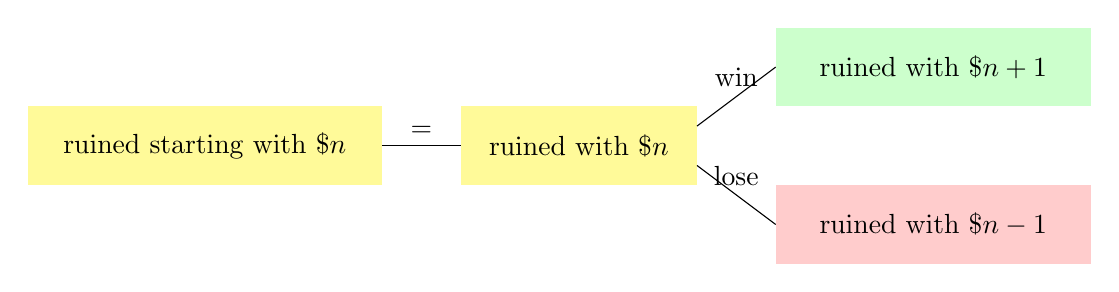
\begin{tikzpicture}
    \fill[color=yellow!40!white] (-4.5,2) rectangle (0,3) node[pos=.5] {\color{black}ruined starting with $\$n$};
    \draw (0,2.5) -- (1,2.5) node[pos=.5,above] {$=$};
    \fill[color=yellow!40!white] (1,2) rectangle (4,3) node[pos=.5] {\color{black}ruined with $\$n$};
    \draw (4,2.75) -- (5,3.5) node[pos=.5,above] {win};
    \fill[color=green!20!white] (5,3) rectangle (9,4) node[pos=.5] {\color{black}ruined with $\$n+1$};
    \draw (4,2.25) -- (5,1.5) node[pos=.5,above] {lose};
    \fill[color=red!20!white] (5,1) rectangle (9,2) node[pos=.5] {\color{black}ruined with $\$n-1$};
\end{tikzpicture}	
\end{center}


The two boxes on the left are very important. The crucial idea is to realize that it doesn't matter when the gambler has $\$n$. If s/he has $\$n$ at two different points in time, then the probability of becoming ruined is the same. \\

This mind map, shows us that we can relate $p_n$, $p_{n+1}$ and $p_{n-1}$.\\

The rest of the modelling will be left as a practice problem.

\end{example}


\begin{video}
\begin{itemize}
	\item \qrvideo{https://youtu.be/Rr2iSKlengg}
\end{itemize}	
\end{video}


\hfill


\submodule{Population Models}

We have modelled populations using differential equations. Populations can be modelled using both differential or difference equations. Which kind of equations to use depends on the goal of the model and the assumptions that we make. 

Below we'll see an example of a population model using difference equations.


\begin{example}

Model a population of mosquitoes, who reproduce at specific times of the year.

\paragraph{Step 1.} The goal is to model the population, so we define
\begin{itemize}
	\item $p(t) = $ population of mosquitoes at time $t$.
\end{itemize}



\paragraph{Step 2.} We create a mind map for this problem.

\begin{center}
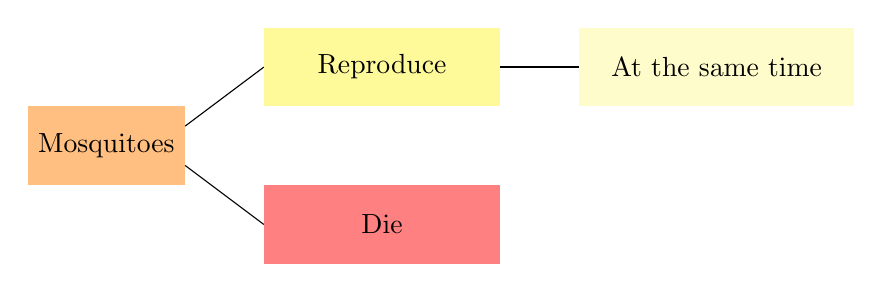
\begin{tikzpicture}
    \fill[color=orange!50!white] (-4.5,2) rectangle (-2.5,3) node[pos=.5] {\color{black}Mosquitoes};
    \draw (-2.5,2.75) -- (-1.5,3.5);
    \fill[color=yellow!40!white] (-1.5,3) rectangle (1.5,4) node[pos=.5] {\color{black}Reproduce};
    \draw (-2.5,2.25) -- (-1.5,1.5);
    \fill[color=red!50!white] (-1.5,1) rectangle (1.5,2) node[pos=.5] {\color{black}Die};
    \draw (1.5,3.5) -- (2.5,3.5);
    \fill[color=yellow!20!white] (2.5,3) rectangle (6,4) node[pos=.5] {\color{black}At the same time};
\end{tikzpicture}
\end{center}



\paragraph{Step 3.} Given that the mosquito population all reproduces at the same time, we don't need to track the population at all times $t$.

So we can assume that the mosquito population doesn't change (much) between seasons, and we change our objective function from $p(t)$ to $p_n$:
\begin{itemize}
	\item $p_n = $ population of mosquitoes at the beginning of season $n$.
\end{itemize}

We understand that mosquitoes die in between seasons, but in this model, we only count the deaths at the beginning of each season. \\

The next assumption is that the number of nymphs (baby mosquitoes) is proportional to the number of mosquitoes in the beginning of the season.

Similarly, the number of deaths is proportional to the number of mosquitoes in the beginning of the season. Also observe that mosquitoes only live for one season, which means that the proportionality constant $\mu > 1$.



\paragraph{Step 4.} So our model is
\begin{itemize}
	\item $p_n = $ population of mosquitoes at the beginning of season $n$.
	\item $p_{n+1} = r p_n - \mu p_n = (r-\mu)p_n$;
	\item $r = $ the average number of nymphs per per mosquito per season;
	\item $\mu = $ the average number of deaths per mosquito per season;
	\item $\mu > 1$, which means that each mosquito itself dies (at the end of the seasons if not earlier), but also some of its nymphs will die.
\end{itemize}

\end{example}

\begin{video}
\begin{itemize}
	\item \qrvideo{https://youtu.be/qmm9GPhA1MY}
\end{itemize}	
\end{video}

